%%%%%%%%%%%%%%%%%%%%%%%%%%%%% Define Article %%%%%%%%%%%%%%%%%%%%%%%%%%%%%%%%%%
\documentclass{article}
%%%%%%%%%%%%%%%%%%%%%%%%%%%%%%%%%%%%%%%%%%%%%%%%%%%%%%%%%%%%%%%%%%%%%%%%%%%%%%%

%%%%%%%%%%%%%%%%%%%%%%%%%%%%% Using Packages %%%%%%%%%%%%%%%%%%%%%%%%%%%%%%%%%%
\usepackage[T1]{fontenc}
\usepackage[utf8]{inputenc}
\usepackage{listings, xcolor}
\usepackage{parskip}
\usepackage{hyperref}
\usepackage{amsmath}
\usepackage{amssymb}
\usepackage{graphicx}
\usepackage{geometry}
\usepackage{float}
\usepackage{import}
\usepackage{tabularx}
\usepackage{booktabs}
\usepackage{longtable}
\usepackage{array}
\usepackage{ragged2e}
\usepackage{pdflscape}
\usepackage[english,italian]{babel}
\selectlanguage{italian}


\graphicspath{{figures/}{../figures/}}

\geometry{a4paper, margin=3cm}

% \lstset{
%   frame = shadowbox,
%   basicstyle = \small\ttfamily,
%   mathescape = true,
%   numbers = left,
%   commentstyle = \itshape\color{gray},
%   columns = flexible,
%   keepspaces = true,
%   moredelim = [l]{//}
% }
%
% TEST CODICE
% --- Nel preambolo del main.tex ---
\usepackage{listings}
\usepackage{xcolor}
\usepackage{inconsolata}

\definecolor{codebg}{HTML}{F7F7F7}
\definecolor{codeframe}{HTML}{D9D9D9}
\definecolor{codecomment}{HTML}{2E7D32}
\definecolor{codekeyword}{HTML}{003C8F}
\definecolor{codestring}{HTML}{B85C00}
\definecolor{codenumber}{HTML}{777777}
\definecolor{codeidentifier}{HTML}{222222}

\lstdefinelanguage{PostgreSQL}{
  language=SQL,
  morekeywords={
    GENERATED, ALWAYS, AS, IDENTITY, IF, EXISTS, CASCADE, RESTRICT,
    RETURNS, TRIGGER, FUNCTION, BEGIN, END, LANGUAGE, plpgsql
  },
  sensitive=false
}

\lstdefinestyle{dbstyle}{
  language=PostgreSQL,
  backgroundcolor=\color{codebg},
  basicstyle=\ttfamily\small,
  keywordstyle=\color{codekeyword}\bfseries,
  commentstyle=\color{codecomment}\itshape,
  stringstyle=\color{codestring},
  identifierstyle=\color{codeidentifier},
  numberstyle=\scriptsize\color{codenumber},
  numbers=left,
  numbersep=8pt,
  stepnumber=1,
  showstringspaces=false,
  showspaces=false,
  showtabs=false,
  breaklines=true,
  breakatwhitespace=true,
  columns=fullflexible,
  keepspaces=true,
  frame=single,
  rulecolor=\color{codeframe},
  frameround=tttt,
  framesep=6pt,
  xleftmargin=10pt,
  xrightmargin=4pt,
  tabsize=2,
  captionpos=b
}

\lstset{
  style=dbstyle,
  literate=
    {à}{{\`a}}1
    {è}{{\`e}}1
    {é}{{\'e}}1
    {ì}{{\`i}}1
    {ò}{{\`o}}1
    {ù}{{\`u}}1
}

%%%%%%%%%%%%%%%%%%%%%%%%%%%%%% Title & Author %%%%%%%%%%%%%%%%%%%%%%%%%%%%%%%%
\begin{document}
\begin{titlepage}
  \begin{center}
    \vspace*{0.8cm}

    {\LARGE\scshape Università degli Studi di Udine\par}
    \vspace{0.7em}
    {\Large\scshape Dipartimento di Scienze Matematiche, Informatiche e Fisiche\par}
    \vspace{1.2em}
    {\normalsize Anno accademico 2025/2026\par}

    \vspace{2em}
    
\includegraphics[width=0.35\textwidth]{imgs/LogoUniUd.png}
    \vspace{2em}

    \rule{\textwidth}{0.5pt}\par
    \vspace{1.2em}
    {\LARGE\bfseries Basi di Dati e Sistemi Informativi\par}
    \vspace{0.6em}
    {\Large Relazione di progetto\par}
    \vspace{0.4em}
    {\normalsize Esercizio 3 -- Progettazione concettuale di una rete bancaria informatizzata\par}
    \vspace{1.2em}
    \rule{\textwidth}{0.5pt}
  \end{center}

  \vspace{3em}

  \noindent
  \begin{minipage}{0.6\textwidth}
    \textbf{Autori}\par
    Ciscato Pajello Leonardo - 167770\par
    Trentin Tommaso -- 167340\par
    Cuna Davide -- 168363\par
    Zita Andi - 167775\par
  \end{minipage}
  \begin{minipage}{0.39\textwidth}
    \raggedleft
    \textbf{Mail}\par
    cistatopajello.leonardo@spes.uniud.it\par
    trentin.tommaso@spes.uniud.it\par
    cuna.davide@spes.uniud.it\par
    zita.andi@spes.uniud.it\par
  \end{minipage}

  \vfill

  \begin{center}
    \normalsize \today
  \end{center}
\end{titlepage}
%%%%%%%%%%%%%%%%%%%%%%%%%%%%%%%%%%%%%%%%%%%%%%%%%%%%%%%%%%%%%%%%%%%%%%%%%%%%%%%
\newpage
\tableofcontents
\newpage

% !TeX root = ../main.tex

\section{Descrizione del problema}
Si vuole progettare una base di dati relativa ad una \textbf{rete bancaria informatizzata}, costituita da un consorzio di banche 
che condividono sportelli automatici(Bancomat). L'obiettivo è modellare il sistema per gestire le relazioni tra banche, filiali,
dipendenti, clienti, conti correnti e operazioni bancarie, includendo la gestione delle carte Bancomat e i relativi costi di commissione.


\section{Analisi dei requisiti}

\subsection{Glossario}
Di seguito sono riportati i termini e le definizioni utilizzate nel progetto, con lo scopo di chiarire i tecnicismi e garantire una comprensione
uniforme del contenuto, individuando inoltre sinonimi e riferimenti comuni tra i termini.

\begin{table}[H]
  \centering
  \footnotesize
  \renewcommand{\arraystretch}{1.0}
  \setlength{\tabcolsep}{3pt}
  \begin{tabularx}{\textwidth}{@{}
      >{\raggedright\arraybackslash}p{2.3cm}
      >{\raggedright\arraybackslash}X
      >{\raggedright\arraybackslash}p{2.6cm}
      >{\raggedright\arraybackslash}p{3.2cm}
    @{}}
    \toprule
    \textbf{Termine} & \textbf{Descrizione} & \textbf{Sinonimi} & \textbf{Collegamenti} \\
    \midrule
    Consorzio & Insieme di banche che condividono un insieme di sportelli automatizzati. & - & Banca, Sportello automatizzato \\
    \midrule

    Banca & Ente individuato da un codice e dotato di un nome; possiede filiali e impiegati e stabilisce i costi dei prelievi effettuati presso sportelli automatizzati del consorzio o di altre banche. & - & Consorzio, Filiale, Impiegato \\
    \midrule

    Filiale & Sede di una banca, individuata da un codice e caratterizzata da un indirizzo; possiede conti, postazioni di cassa e sportelli automatizzati e può rilasciare carte Bancomat. & - & Banca, Impiegato, Conto, Cassa, Sportello automatizzato, Carta Bancomat \\
    \midrule

    Impiegato & Persona di cui si conoscono nome, indirizzo dell'abitazione e data di assunzione; presta servizio presso filiali della stessa banca, con permanenza minima di un mese per filiale. & - & Banca, Filiale, Cliente \\
    \midrule

    Cliente & Persona di cui si conoscono nome, indirizzo e codice fiscale, che la identifica univocamente; può essere titolare di uno o più conti e possedere una o più carte Bancomat; può anche essere impiegato della stessa banca. & - & Conto, Carta Bancomat, Impiegato \\
    \midrule

    Conto & Rapporto bancario relativo a uno o più clienti, con data di apertura, eventuale data di estinzione e, se ancora aperto, ammontare totale. & - & Cliente, Filiale, Carta Bancomat, Operazione bancaria \\
    \midrule

    Carta Bancomat & Carta associata a uno dei conti del cliente, identificata univocamente dalla password e caratterizzata da un limite di spesa giornaliero e da un limite di spesa mensile. & - & Cliente, Conto, Filiale \\
    \midrule

    Cassa & Punto operativo della filiale presso cui si possono eseguire operazioni bancarie; dispone di una quantità di denaro disponibile aggiornata in caso di depositi e prelievi. & Postazione di cassa & Filiale, Operazione bancaria \\
    \midrule

    Sportello automatizzato & Dispositivo automatico presso cui si possono eseguire operazioni bancarie; dispone di una quantità di denaro disponibile ed è condiviso nell'ambito del consorzio. Consente deposito, saldo, lista movimenti e prelievo. & Sportello Bancomat, Stazione automatizzata & Consorzio, Filiale, Operazione bancaria \\
    \midrule

    Operazione bancaria & Operazione eseguita in una certa data e a una certa ora, relativa a un dato conto e svolta presso una cassa o uno sportello automatizzato. & Operazione & Conto, Cassa, Sportello automatizzato \\
    \bottomrule
  \end{tabularx}
  \caption{Glossario dei termini}
  \label{tab:glossario}
\end{table}

\subsection{Strutturazione dei requisiti in gruppi di frasi omogenee}
In questa fase si riorganizzano le frasi del progetto in base ai loro concetti, in modo da ottenere un'organizzazione migliore per il lavoro futuro.

\paragraph{Frasi di carattere generale}
Si vuole progettare una base di dati relativa ad una rete bancaria informatizzata. La rete bancaria è costituita da un consorzio di banche che condivide un insieme di sportelli automatizzati, ossia gli sportelli Bancomat.
\paragraph{Frasi relative alle banche}
Ogni banca è individuata da un codice, ha un proprio nome, un insieme di filiali ed un insieme di impiegati. Alle operazioni di prelievo ogni banca associa due diversi costi: uno per le operazioni di prelievo eseguite presso stazioni automatizzate di banche appartenenti al consorzio e un altro per operazioni eseguite presso stazioni automatizzate di altre banche.

\paragraph{Frasi relative agli impiegati}
Di ogni impiegato vogliamo conoscere il nome, l'indirizzo dell'abitazione e la data di assunzione. Nel corso della vita lavorativa, un impiegato può prestare servizio in diverse filiali della stessa banca, rispettando il vincolo di una permanenza minima di un mese in una filiale.

\paragraph{Frasi relative alle filiali}
Ogni filiale è caratterizzata da un codice e possiede un indirizzo, dei propri conti, delle postazioni di cassa e degli sportelli automatizzati; può, inoltre, rilasciare delle carte Bancomat.

\paragraph{Frasi relative ai conti}
Ogni conto è relativo ad uno o più clienti ed è caratterizzato da una data di apertura, da un'eventuale data di estinzione e (se ancora aperto) da un ammontare totale.

\paragraph{Frasi relative alle carte Bancomat}
Ogni carta Bancomat è identificata univocamente dalla password ed è contraddistinta da un limite di spesa giornaliero e da un limite di spesa mensile (tali limiti possono variare da una carta all'altra).

\paragraph{Frasi relative ai clienti}
Ogni cliente ha un nome, un indirizzo e un numero di codice fiscale che lo identifica univocamente. Un cliente può possedere una o più carte Bancomat, ognuna associata ad uno dei suoi conti. Un cliente della banca può anche essere un impiegato della stessa. In tal caso, non ha alcun costo di gestione per le operazioni eseguite presso le filiali della banca stessa o presso gli sportelli automatizzati del consorzio a cui la banca appartiene.

\paragraph{Frasi relative alle interfacce (casse e sportelli)}
Ogni cassa o sportello automatizzato ha una certa quantità di denaro disponibile, che viene aggiornata in caso di depositi/prelievi. Ovviamente non è possibile effettuare prelievi superiori al denaro disponibile. Sia presso le casse sia presso gli sportelli automatizzati è possibile eseguire operazioni bancarie, le quali avvengono in una certa data ad una certa ora e sono relative ad un dato conto. Attraverso uno sportello automatizzato è possibile effettuare operazioni di deposito, saldo, lista movimenti e prelievo.

\subsection{Lista delle operazioni}

\begin{table}[H]
  \centering
  \begin{tabular}{|c|p{9cm}|c|}
    \hline
    \# & Descrizione & Frequenza stimata \\
    \hline
    1 & Informazioni di un'interfaccia (compreso \# operazioni effettuate) & $\sim 500$ / giorno \\
    \hline
    2 & Inserimento di un'operazione su un'interfaccia, da conto preesistente & $\sim 50{.}000$ / giorno \\
    \hline
    3 & Assunzione di un impiegato in una data filiale & $\sim 0{,}5$ / giorno \\
    \hline
    4 & Trasferimento di un impiegato in una filiale e controllo vincoli temporali & $\sim 0{,}1$ / giorno \\
    \hline
    5 & Licenziamento di un impiegato & $\sim 0{,}011$ / giorno \\
    \hline
    6 & Trovare il cliente con l'ammontare complessivo dei conti correnti intestati maggiore & $\sim 0{,}033$ / giorno \\
    \hline
    7 & Trovare le filiali con solo operazioni di ammontare $> 20$ & $\sim 0{,}033$ / giorno \\
    \hline
    8 & Trovare impiegati-clienti con almeno un conto aperto da 13 anni & $\sim 0{,}033$ / giorno \\
    \hline
    9 & Trovare coppie di clienti che hanno cc in esattamente gli stessi insiemi di filiali & $\sim 0{,}033$ / giorno \\
    \hline
  \end{tabular}
  \caption{Operazioni e frequenze stimate}
\end{table}

\subsection{Volumi dei dati e tavole degli accessi}

Dall'analisi emerge che il carico del sistema è dominato dall'inserimento delle operazioni bancarie, con una frequenza stimata di circa \(50{.}000\) esecuzioni al giorno. Di conseguenza, i costrutti con volume più elevato risultano essere \textbf{Operazione} e le relative associazioni, con cardinalità nell'ordine di \(182{.}500{.}000\) occorrenze su orizzonte decennale. Anche \textbf{Conto}, \textbf{CartaBancomat}, \textbf{Cliente} e le relazioni a essi collegate presentano volumi rilevanti e sono quindi stati considerati con particolare attenzione nelle scelte di indicizzazione.

Le tavole degli accessi mostrano inoltre che le operazioni di consultazione più frequenti coinvolgono in prevalenza \textbf{Interfaccia}, mentre le interrogazioni analitiche meno frequenti richiedono join tra più relazioni, come nel caso di \textbf{Cliente}, \textbf{Conto}, \textbf{Intestato\_A}, \textbf{Filiale} e \textbf{PrestaServizioIn}. Queste stime hanno giustificato l'introduzione di indici sulle principali chiavi esterne e sugli attributi maggiormente coinvolti nelle selezioni e nei collegamenti tra tabelle.

\begin{table}[H]
  \centering
  \begin{tabular}{|l|c|}
    \hline
    Costrutto & Volume stimato \\
    \hline
    Banca & 5 \\
    Filiale & 100 \\
    Interfaccia & 500 \\
    Cliente & 50{.}000 \\
    Persona & 51{.}000 \\
    Impiegato & 1{.}000 \\
    Conto & 60{.}000 \\
    CartaBancomat & 55{.}000 \\
    Operazione & 182{.}500{.}000 \\
    \hline
  \end{tabular}
  \caption{Volumi stimati dei principali costrutti}
\end{table}

\begin{table}[H]
  \centering
  \begin{tabular}{|c|c|l|c|c|}
    \hline
    \textbf{Operazione} & \textbf{Versione} & \textbf{Concetto / Costrutto} & \textbf{Accessi} & \textbf{Tipo} \\
    \hline
    1 & con counter & Interfaccia (E) & 1 & L \\
    \hline
    1 & senza counter & Interfaccia (E) & 1 & L \\
    1 & senza counter & Effettua (R) & 365000 & L \\
    1 & senza counter & Operazione (E) & 365000 & L \\
    \hline
    2 & con counter & Operazione (E) & 1 & S \\
    2 & con counter & Relativo\_a (R) & 1 & S \\
    2 & con counter & Conto (E) & 1 & S \\
    2 & con counter & Effettua (R) & 1 & S \\
    2 & con counter & Interfaccia (E) & 1 & S \\
    \hline
    2 & senza counter & Operazione (E) & 1 & S \\
    2 & senza counter & Relativo\_a (R) & 1 & S \\
    2 & senza counter & Conto (E) & 1 & S \\
    2 & senza counter & Effettua (R) & 1 & S \\
    2 & senza counter & Interfaccia (E) & 1 & S \\
    \hline
  \end{tabular}
  \caption{Confronto degli accessi per le operazioni 1 e 2 con e senza contatore del numero di operazioni per interfaccia}
  \label{tab:counter_accessi}
\end{table}

La tabella mostra che l'introduzione del contatore \textit{numeroOperazioni} nell'entità \textbf{Interfaccia} è giustificata soprattutto dall'operazione 1, che richiede la visualizzazione
delle informazioni di un'interfaccia comprensive del numero di operazioni effettuate.

Con il contatore memorizzato, tale informazione si ottiene con un solo accesso all'entità \textbf{Interfaccia}. Senza contatore, invece, è necessario attraversare la relazione
\textbf{Effettua} e considerare tutte le occorrenze di \textbf{Operazione} associate alla singola interfaccia, con un costo molto più elevato, pari a
centinaia di migliaia di accessi nel caso medio stimato.

L'operazione 2, pur essendo molto frequente, mantiene un costo sostanzialmente costante anche in presenza del contatore, poiché l'aggiornamento del valore può essere eseguito contestualmente
all'inserimento della nuova operazione. Di conseguenza, il contatore introduce una rindondanza controllata, ma consente un forte miglioramento nelle interrogazioni di lettura più sensibili,
risultando quindi una scelta proggettuale conveniente.

% !TeX root = ../main.tex

\section{Progettazione Concettuale}
In questa fase si individuano e si modellano i concetti rilevanti del dominio applicativo, indipendentemente dagli aspetti implementativi o tecnologici. L'obiettivo è costruire uno schema \textbf{Entità-Relazione} che descriva in modo chiaro le entità del sistema, i loro attributi, le associazioni tra esse e i vincoli principali imposti dalla traccia.

La progettazione è stata sviluppata in due momenti distinti: una prima modellazione completa del dominio mediante uno schema ER esteso, e una successiva ristrutturazione del modello, finalizzata a semplificarne la struttura senza alterarne il contenuto informativo essenziale.

\subsection{Schema Entità-Relazioni (ER)}
\begin{figure}[H]
  \begin{center}
    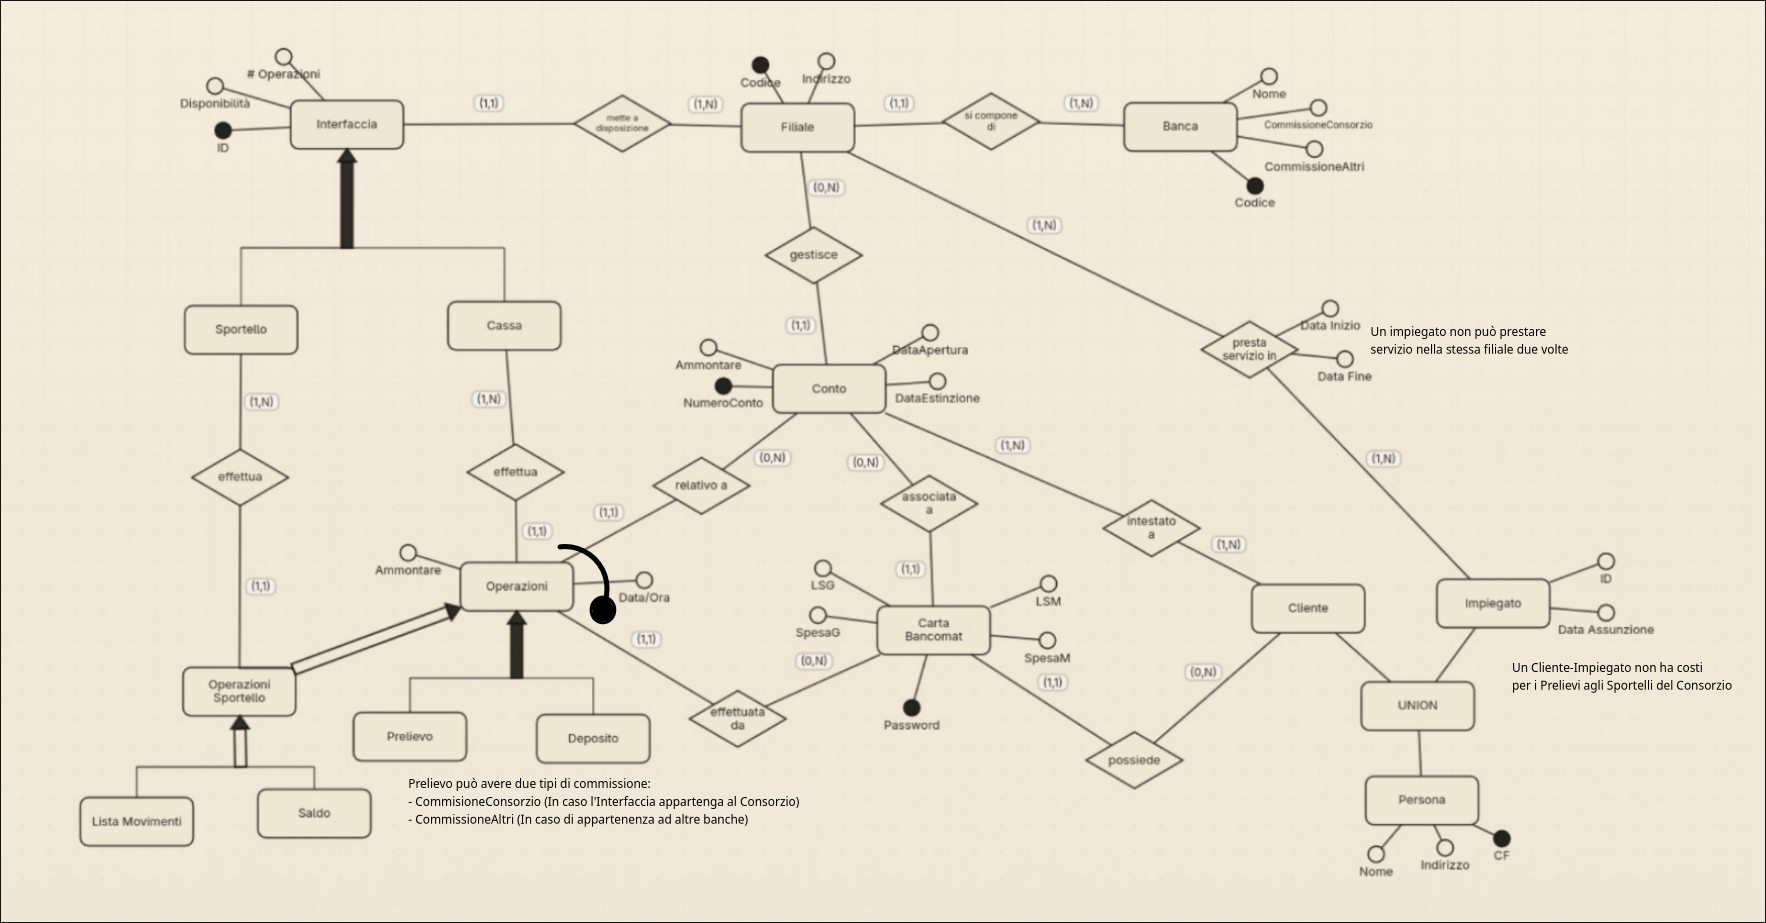
\includegraphics[width=0.95\textwidth]{../imgs/modelloER.png}
  \end{center}
  \caption{Schema Entità-Relazione iniziale del Consorzio Bancario}
  \label{fig:er_model}
\end{figure}

\subsection{Analisi dello schema}
Lo schema concettuale descrive una rete bancaria informatizzata costituita da più banche appartenenti a un medesimo consorzio e dotate di filiali, impiegati, conti, carte Bancomat e postazioni operative per l'esecuzione delle operazioni bancarie.

Nel modello iniziale si è scelto di rappresentare in modo esplicito alcune differenze semantiche attraverso gerarchie di specializzazione, in particolare per distinguere i diversi tipi di interfaccia e i diversi tipi di operazione.

\subsubsection{Entità e gerarchie}

\begin{itemize}
  \item \textbf{Banca}: ente bancario appartenente al consorzio, identificato da un codice e dotato di un nome. Per ciascuna banca vengono inoltre memorizzate le commissioni applicate ai prelievi effettuati presso sportelli del consorzio o presso sportelli di altre banche.\\
  Attributi: \textit{Codice} (chiave primaria), \textit{Nome}, \textit{CommissioneConsorzio}, \textit{CommissioneAltri}.

  \item \textbf{Filiale}: sede operativa di una banca. Ogni filiale è caratterizzata da un proprio codice e da un indirizzo; presso di essa vengono gestiti i conti, lavorano gli impiegati e sono messe a disposizione le interfacce operative.\\
  Attributi: \textit{Codice} (chiave primaria), \textit{Indirizzo}.

  \item \textbf{Persona}: entità generale che raccoglie le informazioni anagrafiche comuni ai soggetti del sistema.\\
  Attributi: \textit{CF} (chiave primaria), \textit{Nome}, \textit{Indirizzo}.

  \item \textbf{Cliente}: entità che rappresenta i soggetti intestatari di conti e possessori di carte Bancomat.\\
  Attributi: ereditati da \textbf{Persona}.

  \item \textbf{Impiegato}: entità che rappresenta i dipendenti della banca.\\
  Attributi: \textit{ID}, \textit{Data Assunzione}, oltre agli attributi comuni ereditati da \textbf{Persona}.

  \item \textbf{Conto}: rapporto bancario relativo a uno o più clienti e gestito da una filiale.\\
  Attributi: \textit{Numero Conto} (chiave primaria), \textit{Data Apertura}, \textit{Data Estinzione}, \textit{Ammontare}.

  \item \textbf{Carta Bancomat}: strumento associato a un conto e utilizzabile per l'esecuzione delle operazioni bancarie.\\
  Attributi: \textit{Password} (chiave primaria), \textit{Limite Spesa Giornaliero(LSG)}, \textit{Limite Spesa Mensile(LSM)}, \textit{SpesaG}, \textit{SpesaM}.

  \item \textbf{Interfaccia}: postazione operativa presso cui possono essere eseguite operazioni bancarie.\\
  Attributi: \textit{ID} (chiave primaria), \textit{Disponibilità}, \textit{\#Operazioni}.

  \item \textbf{Cassa}: specializzazione di \textbf{Interfaccia}. Rappresenta una postazione di cassa fisica presente presso una filiale.\\
  Attributi: ereditati da \textbf{Interfaccia}.

  \item \textbf{Sportello}: specializzazione di \textbf{Interfaccia}. Rappresenta uno sportello automatico.\\
  Attributi: ereditati da \textbf{Interfaccia}.

  \item \textbf{Operazioni}: entità che rappresenta una generica operazione bancaria eseguita su un conto.\\
  Attributi: \textit{Data/Ora}, \textit{Ammontare}.

  \item \textbf{Prelievo}: specializzazione di \textbf{Operazioni}.\\
  Attributi: ereditati da \textbf{Operazioni}.

  \item \textbf{Deposito}: specializzazione di \textbf{Operazioni}.\\
  Attributi: ereditati da \textbf{Operazioni}.

  \item \textbf{Operazioni Sportello}: specializzazione di \textbf{Operazioni} che raccoglie le operazioni specificamente modellate per lo sportello automatico.\\
  Attributi: ereditati da \textbf{Operazioni}.

  \item \textbf{Saldo}: specializzazione di \textbf{Operazioni Sportello}.\\
  Attributi: ereditati da \textbf{Operazioni Sportello}.

  \item \textbf{Lista Movimenti}: specializzazione di \textbf{Operazioni Sportello}.\\
  Attributi: ereditati da \textbf{Operazioni Sportello}.
\end{itemize}

Nel modello iniziale:
\begin{itemize}
  \item \textbf{Interfaccia} è specializzata in \textbf{Cassa} e \textbf{Sportello} mediante una gerarchia \textbf{totale e disgiunta};
  \item \textbf{Operazioni} è specializzata in \textbf{Prelievo}, \textbf{Deposito} e \textbf{Operazioni Sportello} mediante una gerarchia \textbf{totale e disgiunta};
  \item \textbf{Operazioni Sportello} è ulteriormente specializzata in \textbf{Saldo} e \textbf{Lista Movimenti} mediante una gerarchia \textbf{parziale e disgiunta};
  \item \textbf{Persona} raccoglie gli attributi comuni a \textbf{Cliente} e \textbf{Impiegato}, consentendo di rappresentare il caso in cui uno stesso soggetto possa appartenere a entrambi i ruoli.
\end{itemize}

\subsubsection{Relazioni}

\begin{itemize}
  \item \textbf{Si compone di} (\textbf{Banca} $\rightleftarrows$ \textbf{Filiale}): rappresenta l'appartenenza di una filiale a una banca.\\
  Cardinalità:
  \begin{itemize}
    \item una banca si compone di una o più filiali \((1,N)\);
    \item una filiale appartiene a una sola banca \((1,1)\).
  \end{itemize}

  \item \textbf{Mette a disposizione} (\textbf{Filiale} $\rightleftarrows$ \textbf{Interfaccia}): associa a ciascuna filiale le interfacce operative presenti presso di essa.\\
  Cardinalità:
  \begin{itemize}
    \item una filiale mette a disposizione una o più interfacce \((1,N)\);
    \item un'interfaccia appartiene a una sola filiale \((1,1)\).
  \end{itemize}

  \item \textbf{Gestisce} (\textbf{Filiale} $\rightleftarrows$ \textbf{Conto}): collega ciascun conto alla filiale che lo gestisce.\\
  Cardinalità:
  \begin{itemize}
    \item una filiale può gestire zero o più conti \((0,N)\);
    \item un conto è gestito da una sola filiale \((1,1)\).
  \end{itemize}

  \item \textbf{Intestata a} (\textbf{Conto} $\rightleftarrows$ \textbf{Cliente}): rappresenta l'intestazione del conto a uno o più clienti.\\
  Cardinalità:
  \begin{itemize}
    \item un conto è intestato a uno o più clienti \((1,N)\);
    \item un cliente può essere intestatario di uno o più conti \((1,N)\).
  \end{itemize}

  \item \textbf{Associata a} (\textbf{Carta Bancomat} $\rightleftarrows$ \textbf{Conto}): collega ogni carta al conto cui essa è riferita.\\
  Cardinalità:
  \begin{itemize}
    \item una carta Bancomat è associata a un solo conto \((1,1)\);
    \item un conto può avere zero o più carte associate \((0,N)\).
  \end{itemize}

  \item \textbf{Possiede} (\textbf{Cliente} $\rightleftarrows$ \textbf{Carta Bancomat}): rappresenta il possesso della carta da parte del cliente.\\
  Cardinalità:
  \begin{itemize}
    \item un cliente può possedere zero o più carte Bancomat \((0,N)\);
    \item una carta Bancomat è posseduta da un solo cliente \((1,1)\).
  \end{itemize}

  \item \textbf{Relativo a} (\textbf{Operazioni} $\rightleftarrows$ \textbf{Conto}): collega ogni operazione al conto cui essa si riferisce.\\
  Cardinalità:
  \begin{itemize}
    \item un conto può essere coinvolto in zero o più operazioni \((0,N)\);
    \item ogni operazione è relativa a un solo conto \((1,1)\).
  \end{itemize}

  \item \textbf{Effettuata da} (\textbf{Operazioni} $\rightleftarrows$ \textbf{Carta Bancomat}): collega una operazione alla carta utilizzata.\\
  Cardinalità:
  \begin{itemize}
    \item un'operazione deve essere effettuata da una sola carta Bancomat \((1,1)\);
    \item una carta Bancomat può essere utilizzata per zero o più operazioni \((0,N)\).
  \end{itemize}

  \item \textbf{Effettua} (\textbf{Cassa} $\rightleftarrows$ \textbf{Operazioni}): indica le operazioni eseguite tramite una cassa.\\
  Cardinalità:
  \begin{itemize}
    \item una cassa può effettuare una o più operazioni \((1,N)\);
    \item ogni operazione è eseguita da una sola cassa \((1,1)\).
  \end{itemize}

  \item \textbf{Effettua} (\textbf{Sportello} $\rightleftarrows$ \textbf{Operazioni Sportello}): indica le operazioni eseguite tramite sportello automatico.\\
  Cardinalità:
  \begin{itemize}
    \item uno sportello può effettuare una o più operazioni \((1,N)\);
    \item ogni operazione di sportello è eseguita da un solo sportello \((1,1)\).
  \end{itemize}

  \item \textbf{Presta servizio in} (\textbf{Impiegato} $\rightleftarrows$ \textbf{Filiale}): rappresenta l'assegnazione dell'impiegato a una filiale.\\
  Cardinalità:
  \begin{itemize}
    \item una filiale impiega uno o più impiegati \((1,N)\);
    \item ciascun impiegato presta servizio in una filiale \((1,N)\).
  \end{itemize}
  Attributi della relazione:
  \begin{itemize}
    \item \textit{DataInizio}: data di inizio del servizio presso la filiale;
    \item \textit{DataFine}: data di termine del servizio presso la filiale.
  \end{itemize}
\end{itemize}

\subsubsection{Attributi derivati e osservazioni}

Nel modello iniziale l'attributo \textit{\#Operazioni} di \textbf{Interfaccia} è da considerarsi \textbf{derivato}, in quanto ricavabile dal conteggio delle operazioni eseguite dalla singola interfaccia.

Anche gli attributi \textit{SpesaG} e \textit{SpesaM} associati alla \textbf{Carta Bancomat} possono essere interpretati come valori mantenuti e aggiornati sulla base delle operazioni registrate in determinati intervalli temporali.

\subsection{Vincoli}
Alcuni vincoli richiesti dalla traccia non sono esprimibili in modo completo mediante il solo formalismo grafico ER e devono quindi essere specificati testualmente.

\begin{itemize}
  \item Un impiegato può prestare servizio solo presso filiali appartenenti alla propria banca.
  \item Un impiegato deve permanere in una filiale per almeno un mese prima di poter essere trasferito.
  \item Un cliente può essere anche impiegato della stessa banca.
  \item Un conto estinto deve avere \textit{Ammontare} nullo oppure pari a zero.
  \item L'importo di un prelievo non può essere superiore alla disponibilità dell'interfaccia presso cui viene effettuato.
  \item L'importo di un prelievo non può superare il limite di spesa giornaliero o mensile della carta Bancomat utilizzata.
  \item Le commissioni associate ai prelievi dipendono dal fatto che lo sportello appartenga a una banca del consorzio oppure a una banca esterna.
  \item Un cliente che sia anche impiegato della stessa banca non sostiene costi di gestione per le operazioni effettuate presso filiali della banca stessa o presso sportelli del consorzio.
\end{itemize}

\subsection{Analisi dei cicli}
Nel modello sono presenti percorsi multipli tra alcune entità, in particolare tra \textbf{Cliente}, \textbf{Conto}, \textbf{Carta Bancomat} e \textbf{Operazioni}. Questi tuttavia, non introducono ambiguità concettuali, poiché ciascuna relazione esprime un significato distinto: l'intestazione del conto, il possesso della carta, l'associazione tra carta e conto e l'esecuzione delle operazioni.

Si può quindi concludere che \textbf{non} emergono cicli problematici dal punto di vista concettuale; le eventuali dipendenze sono controllate tramite cardinalità e vincoli applicativi.

% !TeX root = ../main.tex

\section{Progettazione Logica}

\subsection{Ristrutturazione del modello Entità-Relazione}
A partire dallo schema iniziale è stata effettuata una ristrutturazione del modello con l'obiettivo di ridurre la frammentazione del diagramma e rendere più agevole la successiva traduzione verso il modello logico-relazionale.

La revisione ha riguardato soprattutto i punti in cui il modello originale utilizzava più livelli di specializzazione per rappresentare differenze operative che potevano essere espresse in modo più compatto.

In particolare:
\begin{itemize}
  \item le specializzazioni \textbf{Cassa} e \textbf{Sportello} sono state accorpate nell'unica entità \textbf{Interfaccia}, introducendo l'attributo \textit{Tipo} come discriminante;
  \item la gerarchia di \textbf{Operazioni}, articolata nei sottotipi \textbf{Prelievo}, \textbf{Deposito} e \textbf{Operazioni Sportello}, è stata semplificata in una singola entità \textbf{Operazioni} con attributo \textit{Tipo};
  \item i sottotipi \textbf{Saldo} e \textbf{Lista Movimenti}, originariamente modellati come specializzazioni di \textbf{Operazioni Sportello}, sono stati ricondotti a valori del medesimo attributo \textit{Tipo};
  \item la rappresentazione dei soggetti del sistema è stata resa più lineare attorno all'entità \textbf{Persona}, mantenendo i ruoli di \textbf{Cliente} e \textbf{Impiegato} ma riducendo la complessità grafica complessiva;
\end{itemize}

La ristrutturazione non altera il significato informativo dello schema, ma ne migliora la leggibilità e ne riduce il numero di costrutti specializzati. In questo modo il modello finale risulta più compatto e più facilmente traducibile nello schema logico-relazionale, pur rimanendo coerente con i requisiti della traccia.

\begin{figure}[H]
  \begin{center}
    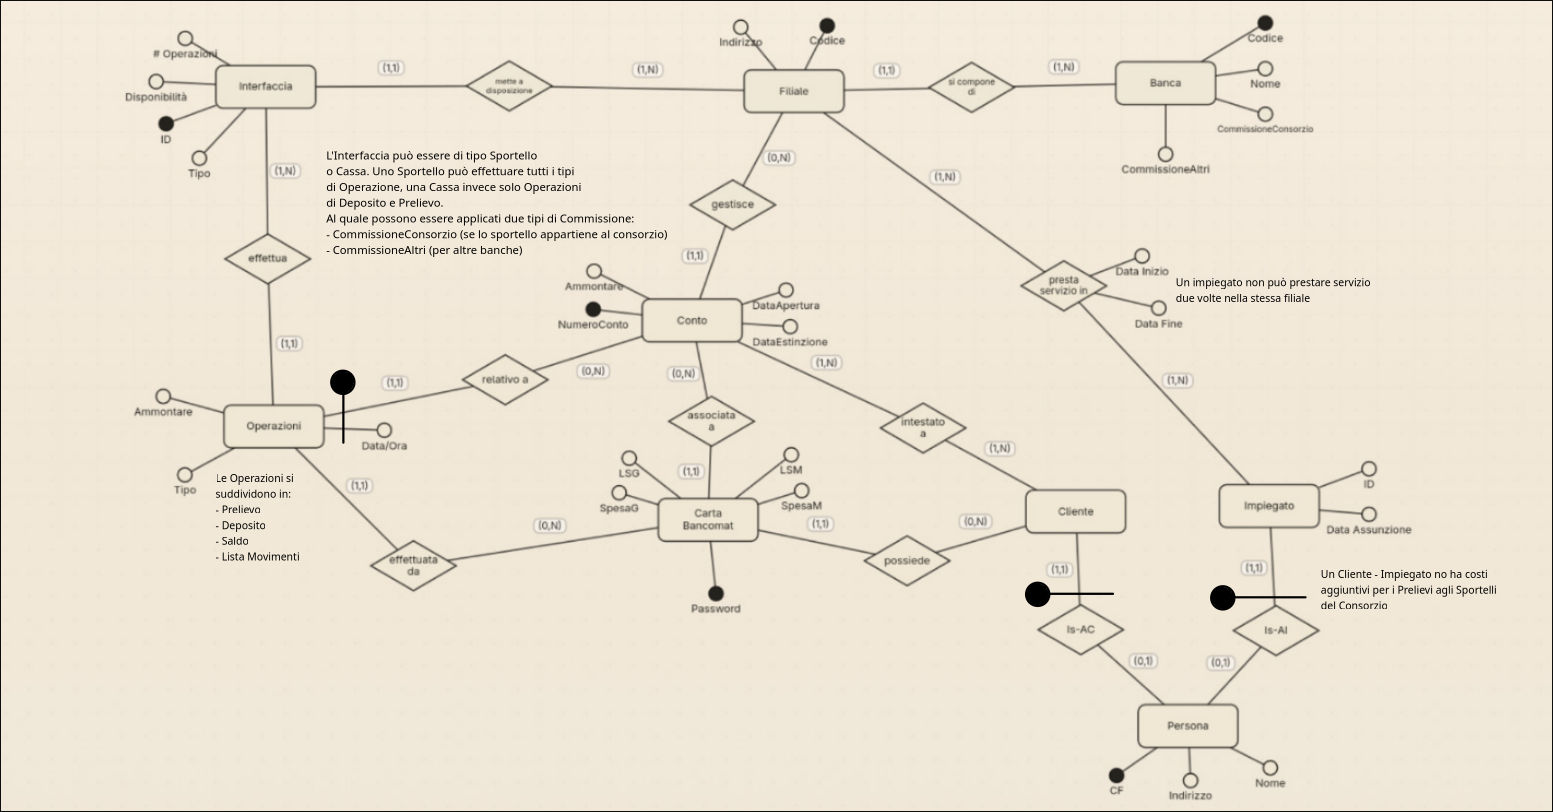
\includegraphics[width=0.95\textwidth]{../imgs/refactorER.png}
  \end{center}
  \caption{Ristrutturazione dello schema Entità-Relazione del Consorzio Bancario}
  \label{fig:ref_er}
\end{figure}


In seguito alla ristrutturazione si procede alla sua traduzione nel modello \textbf{relazionale}. In questa fase, le entità del dominio, le associazioni e i vincoli principali vengono rappresentati mediante relazioni, chiavi primarie, chiavi esterne e, vincoli di integrità.

La traduzione è stata effettuata seguendo i criteri classici:
\begin{itemize}
  \item ogni entità forte è stata trasformata in una relazione;
  \item le relazioni \textit{uno a molti} sono state tradotte riportando la chiave primaria dell'entità dal lato \(1\) come chiave esterna dell'entità dal lato \(N\);
  \item le relazioni \textit{molti a molti} sono state tradotte mediante relazioni autonome;
  \item la generalizzazione \textbf{Persona} -- \textbf{Cliente}/\textbf{Impiegato} è stata realizzata mantenendo una relazione per la superclasse e una per ciascun sottotipo;
  \item le specializzazioni introdotte nel modello concettuale per \textbf{Interfaccia} e \textbf{Operazione} sono state assorbite dall'attributo \textbf{tipo};
\end{itemize}


\subsection{Schema relazionale}

Lo schema logico risultante è il seguente:

\begin{itemize}
  \item \textbf{Banca}(\underline{codiceBanca}, nomeBanca, commissioneAltri, commissioneConsorzio)

  \item \textbf{Filiale}(\underline{codiceFiliale}, indirizzo, \textit{bancaReferente})

  \item \textbf{Persona}(\underline{codiceFiscale}, nome, indirizzo)

  \item \textbf{Cliente}(\underline{\textit{codiceFiscale\_c}})

  \item \textbf{Impiegato}(\underline{\textit{codiceFiscale\_i}}, idImpiegato, dataAssunzione)

  \item \textbf{Conto}(\underline{numeroConto}, dataApertura, dataEstinzione, ammontare, \textit{filialeReferente})

  \item \textbf{Intestato\_A}(\underline{\textit{codiceFiscale\_int}}, \underline{\textit{numeroConto\_int}})

  \item \textbf{CartaBancomat}(\underline{passwordBancomat}, limiteSpesaGiornaliero, limiteSpesaMensile, spesaGiornaliera, spesaMensile, \textit{numeroConto\_cb}, \textit{codiceFiscale\_cb})

  \item \textbf{Interfaccia}(\underline{idInterfaccia}, tipo, disponibilita, numeroOperazioni, \textit{codiceFiliale\_i})

  \item \textbf{Operazione}(\underline{idOperazione}, dataOperazione, oraOperazione, tipo, ammontare, \textit{numeroConto\_o}, \textit{idInterfaccia\_o}, \textit{passwordBancomat})

  \item \textbf{PrestaServizioIn}(\underline{\textit{idImpiegato\_psi}}, \underline{\textit{codiceFiliale\_psi}}, dataInizio, dataFine)
\end{itemize}

Nel precedente schema, gli attributi sottolineati rappresentano le \textbf{chiavi primarie}, mentre quelli in corsivo rappresentano le \textbf{chiavi esterne}.

\subsection{Chiavi esterne e significato delle relazioni}

Le dipendenze referenziali introdotte sono le seguenti:

\begin{itemize}
  \item \textit{bancaReferente} in \textbf{Filiale} referenzia \textbf{Banca}(codiceBanca);
  \item \textit{codiceFiscale\_c} in \textbf{Cliente} referenzia \textbf{Persona}(codiceFiscale);
  \item \textit{codiceFiscale\_i} in \textbf{Impiegato} referenzia \textbf{Persona}(codiceFiscale);
  \item \textit{filialeReferente} in \textbf{Conto} referenzia \textbf{Filiale}(codiceFiliale);
  \item \textit{codiceFiscale\_int} in \textbf{Intestato\_A} referenzia \textbf{Cliente}(codiceFiscale\_c);
  \item \textit{numeroConto\_int} in \textbf{Intestato\_A} referenzia \textbf{Conto}(numeroConto);
  \item \textit{numeroConto\_cb} in \textbf{CartaBancomat} referenzia \textbf{Conto}(numeroConto);
  \item \textit{codiceFiscale\_cb} in \textbf{CartaBancomat} referenzia \textbf{Cliente}(codiceFiscale\_c);
  \item \textit{codiceFiliale\_i} in \textbf{Interfaccia} referenzia \textbf{Filiale}(codiceFiliale);
  \item \textit{numeroConto\_o} in \textbf{Operazione} referenzia \textbf{Conto}(numeroConto);
  \item \textit{idInterfaccia\_o} in \textbf{Operazione} referenzia \textbf{Interfaccia}(idInterfaccia);
  \item \textit{passwordBancomat\_o} in \textbf{Operazione} referenzia \textbf{CartaBancomat}(passwordBancomat);
  \item \textit{idImpiegato\_psi} in \textbf{PrestaServizioIn} referenzia \textbf{Impiegato}(idImpiegato);
  \item \textit{codiceFiliale\_psi} in \textbf{PrestaServizioIn} referenzia \textbf{Filiale}(codiceFiliale).
\end{itemize}

\subsection{Osservazioni sulle scelte di traduzione}

La generalizzazione tra \textbf{Persona}, \textbf{Cliente} e \textbf{Impiegato} è stata mantenuta in modo esplicito, così da poter rappresentare correttamente il caso in cui uno stesso soggetto sia contemporaneamente cliente e impiegato. In questo modo le informazioni anagrafiche comuni sono memorizzate una sola volta nella relazione \textbf{Persona}, evitando ridondanze.

Per l'entità \textbf{Impiegato} è stato introdotto, oltre al codice fiscale ereditato da \textbf{Persona}, anche l'attributo \textit{idImpiegato}, utilizzato come identificatore operativo nelle relazioni di servizio presso le filiali. Tale attributo costituisce una chiave alternativa con vincolo di univocità.

La relazione \textbf{Intestato\_A} realizza l'associazione molti-a-molti tra clienti e conti correnti, in quanto un conto può essere cointestato a più clienti e un cliente può possedere più conti.

L'entità \textbf{CartaBancomat} è stata tradotta in una relazione autonoma collegata sia al conto sia al cliente possessore. Sono stati inoltre mantenuti gli attributi \textit{spesaGiornaliera} e \textit{spesaMensile}, utili al controllo dei limiti operativi della carta.

Le entità \textbf{Cassa} e \textbf{Sportello} del modello concettuale sono state ricondotte alla sola relazione \textbf{Interfaccia}, distinguendo i due casi attraverso l'attributo \textit{tipo}. In modo analogo, i diversi tipi di operazione bancaria sono stati accorpati nella relazione \textbf{Operazione}, ancora una volta tramite l'attributo \textit{tipo}.

L'attributo \textit{ammontare} di \textbf{Operazione} può risultare nullo per operazioni informative come saldo e lista movimenti, mentre assume un valore numerico per depositi e prelievi.

L'attributo \textit{numeroOperazioni} di \textbf{Interfaccia}, pur essendo concettualmente derivabile dal conteggio delle operazioni eseguite, è stato mantenuto nello schema logico in forma memorizzata per motivi di efficienza, delegandone l'aggiornamento automatico alla logica implementativa.

\subsection{Vincoli di integrità non esprimibili direttamente nello schema relazionale}

Alcuni vincoli applicativi non sono esprimibili in modo completo mediante sole chiavi e vincoli referenziali, e richiedono quindi controlli aggiuntivi a livello implementativo:

\begin{itemize}
  \item un impiegato può prestare servizio soltanto presso filiali appartenenti alla banca di riferimento;
  \item un impiegato deve permanere per almeno un mese in una filiale prima di potere essere trasferito;
  \item un impiegato non può essere assegnato nuovamente a una filiale presso cui ha già prestato servizio;
  \item un conto estinto non può essere utilizzato per nuove operazioni;
  \item in caso di estinzione del conto, l'ammontare residuo deve essere nullo oppure pari a zero;
  \item un prelievo non può superare il saldo disponibile del conto;
  \item un prelievo non può superare la disponibilità dell'interfaccia presso cui viene effettuato;
  \item la carta Bancomat utilizzata in un'operazione deve essere associata al conto su cui l'operazione viene eseguita;
  \item l'importo di un prelievo non può eccedere il limite giornaliero o mensile disponibile della carta;
  \item le commissioni sui prelievi dipendono dalla banca proprietaria del conto e dalla banca a cui appartiene l'interfaccia utilizzata;
  \item nel caso in cui un cliente sia anche impiegato della stessa banca, non vengono applicate commissioni per le operazioni effettuate presso filiali della banca stessa o presso sportelli del consorzio.
\end{itemize}

\subsection{Qualità dello schema}
Lo schema risulta regolare e adeguato alla traduzione fisica. La separazione tra \textbf{Persona}, \textbf{Cliente} e \textbf{Impiegato}, così come l'uso di relazioni associative per i legami molti-a-molti, mantiene una struttura coerente con i requisiti della traccia. Alcuni attributi ridondanti sono stati mantenuti consapevolmente per supportare in modo più efficiente controlli e aggiornamenti operativi.

% !TeX root = ../main.tex

\section{Progettazione Fisica}
La progettazione fisica rappresenta la traduzione concreta dello schema logico nel DBMS scelto, nel nostro caso \textbf{PostgreSQL}. In questa fase si definiscono le tabelle effettive, i tipi di dato, i vincoli di integrità esprimibili direttamente nel DDL e gli indici necessari a supportare in modo efficiente le operazioni più frequenti previste dal progetto.

Dal punto di vista operativo, l'infrastruttura del database è stata organizzata mediante una fase iniziale di creazione e reinizializzazione del database, seguita dalla definizione dello schema applicativo \texttt{consorzio}. Tutte le tabelle, i vincoli e la logica successiva vengono infatti collocati all'interno di tale schema, così da mantenere ordinata e separata l'intera base di dati.

\subsection{Scelte implementative e organizzazione dello schema}
La realizzazione fisica è stata organizzata attorno allo schema \texttt{consorzio}, impostato come \texttt{search\_path} di riferimento per gli script SQL. L'inizializzazione prevede la chiusura delle connessioni attive al database, la sua ricreazione e la definizione dello schema applicativo.

\begin{lstlisting}[caption={Inizializzazione del database e dello schema}]
SELECT pg_terminate_backend(pg_stat_activity.pid)
FROM pg_stat_activity
WHERE pg_stat_activity.datname = '${DB_NAME}' AND pid <> pg_backend_pid();

DROP DATABASE IF EXISTS ${DB_NAME};
CREATE DATABASE ${DB_NAME};

create schema if not exists consorzio;
set search_path to consorzio;
\end{lstlisting}

Per quanto riguarda la modellazione dei domini, si è scelto di sfruttare i tipi enumerativi di PostgreSQL per gli attributi che ammettono un insieme chiuso di valori. In particolare, il tipo di interfaccia e il tipo di operazione sono stati modellati tramite \texttt{ENUM}, evitando così l'uso ripetuto di vincoli \texttt{CHECK} sulle stesse colonne e rendendo il dominio dei valori più esplicito a livello di schema.

\begin{lstlisting}[caption={Definizione dei tipi enumerativi}]
create type tipo_interfaccia as enum ('cassa', 'sportello');
create type tipo_operazione as enum ('prelievo', 'deposito', 'saldo', 'lista_movimenti');
\end{lstlisting}

Dal punto di vista dei tipi di dato:
\begin{itemize}
    \item gli identificativi principali del sistema bancario sono stati realizzati prevalentemente come interi autogenerati tramite \texttt{GENERATED ALWAYS AS IDENTITY};
    \item gli attributi descrittivi, come nomi e indirizzi, sono stati modellati con \texttt{VARCHAR};
    \item gli importi monetari, i limiti di spesa e le disponibilità sono stati rappresentati tramite \texttt{NUMERIC(x, 2)}, così da evitare approssimazioni indesiderate mantenendo due cifre dopo la virgola;
    \item le informazioni temporali sono state memorizzate con i tipi \texttt{DATE} e \texttt{TIME}, coerentemente con il modello logico.
\end{itemize}

Queste scelte permettono di mantenere lo schema aderente al modello progettato e, allo stesso tempo, di sfruttare in modo appropriato le caratteristiche offerte da PostgreSQL.

\subsection{Definizione delle tabelle}
Le tabelle sono state implementate seguendo la struttura dello schema logico, distinguendo tra organizzazione bancaria, soggetti del sistema, conti e strumenti di pagamento, interfacce operative e registrazione delle operazioni.

\subsubsection{Organizzazione bancaria}
Le prime due tabelle descrivono la struttura del consorzio bancario: \texttt{banca} rappresenta gli istituti aderenti, mentre \texttt{filiale} modella le sedi operative appartenenti alle singole banche.

\begin{lstlisting}[caption={Tabelle banca e filiale}]
create table banca (
    codiceBanca integer generated always as identity primary key,
    nomeBanca varchar(50) not null,
    commissioneAltri numeric(4, 2) not null,
    commissioneConsorzio numeric(4, 2) not null
);

create table filiale (
    codiceFiliale integer generated always as identity primary key,
    indirizzo varchar(100) not null,
    bancaReferente integer not null,
    foreign key (bancaReferente) references banca(codiceBanca)
);
\end{lstlisting}

In questa fase le commissioni sono memorizzate direttamente nella tabella \texttt{banca}, poiché costituiscono un dato strutturale necessario al successivo calcolo dei costi applicati ai prelievi.

\subsubsection{Soggetti del sistema}
Per rappresentare correttamente il fatto che una stessa persona possa essere cliente, impiegato, oppure entrambe le cose, la generalizzazione \texttt{Persona} -- \texttt{Cliente}/\texttt{Impiegato} è stata mantenuta mediante tabelle distinte collegate tra loro tramite chiavi esterne.

\begin{lstlisting}[caption={Tabelle persona, cliente e impiegato}]
create table persona (
    codiceFiscale varchar(16) primary key,
    indirizzo varchar(100) not null,
    nome varchar(30) not null
);

create table cliente (
    codiceFiscale_c varchar(16) primary key
        references persona(codiceFiscale) ON DELETE CASCADE
);

create table impiegato (
    codiceFiscale_i varchar(16) primary key
        references persona(codiceFiscale) ON DELETE CASCADE,
    idImpiegato integer generated always as identity unique,
    dataAssunzione date not null
);
\end{lstlisting}

L'attributo \texttt{idImpiegato} è stato introdotto come identificatore operativo univoco dell'impiegato. Esso non sostituisce il codice fiscale come chiave primaria della tabella, ma viene utilizzato nelle relazioni operative e nei trigger, risultando più pratico nella gestione interna dei trasferimenti e delle assegnazioni.

La storicizzazione del servizio prestato in filiale è stata implementata tramite la tabella \texttt{presta\_servizio\_in}.

\begin{lstlisting}[caption={Tabella presta\_servizio\_in}]
create table presta_servizio_in (
    idImpiegato_psi integer,
    codiceFiliale_psi integer,
    dataInizio date not null,
    dataFine date,
    primary key (idImpiegato_psi, codiceFiliale_psi),
    foreign key (idImpiegato_psi) references impiegato(idImpiegato) ON DELETE CASCADE,
    foreign key (codiceFiliale_psi) references filiale(codiceFiliale) ON DELETE CASCADE
);
\end{lstlisting}

La tabella registra il legame tra impiegato e filiale, insieme alle date di inizio e fine del servizio. La chiave primaria composta impedisce che la stessa coppia impiegato-filiale venga registrata più di una volta, mentre i vincoli temporali più specifici vengono demandati a controlli aggiuntivi.

\subsubsection{Conti e carte Bancomat}
Il nucleo bancario del progetto è rappresentato dalle tabelle \texttt{conto}, \texttt{intestato\_a} e \texttt{cartaBancomat}. La prima descrive il conto corrente, la seconda realizza la cointestazione tra clienti e conti, mentre la terza modella le carte Bancomat associate a un cliente e a un conto.

\begin{lstlisting}[caption={Tabelle conto e intestato\_a}]
create table conto (
    numeroConto integer generated always as identity primary key,
    dataApertura date not null,
    dataEstinzione date,
    ammontare numeric(17,2),
    filialeReferente integer not null,
    foreign key (filialeReferente) references filiale(codiceFiliale)
);

create table intestato_a (
    codiceFiscale_int varchar(16),
    numeroConto_int integer,
    primary key (codiceFiscale_int, numeroConto_int),
    foreign key (codiceFiscale_int) references cliente(codiceFiscale_c) ON DELETE CASCADE,
    foreign key (numeroConto_int) references conto(numeroConto) ON DELETE CASCADE
);
\end{lstlisting}

\begin{lstlisting}[caption={Tabella cartaBancomat}]
create table cartaBancomat (
    passwordBancomat varchar(25) primary key,
    numeroConto_cb integer not null,
    codiceFiscale_cb varchar(16) not null,

    limiteSpesaGiornaliero numeric(10, 2) not null,
    limiteSpesaMensile numeric(14, 2) not null,

    spesaGiornaliera numeric(10, 2) default 0 not null,
    spesaMensile numeric(14, 2) default 0 not null,

    foreign key (numeroConto_cb) references conto(numeroConto) ON DELETE CASCADE,
    foreign key (codiceFiscale_cb) references cliente(codiceFiscale_c) ON DELETE CASCADE
);
\end{lstlisting}

Nella tabella \texttt{cartaBancomat} sono presenti anche gli attributi \texttt{spesaGiornaliera} e \texttt{spesaMensile}, mantenuti direttamente nel database per consentire controlli rapidi sui limiti operativi senza dover ricalcolare ogni volta lo storico delle operazioni effettuate.

\subsubsection{Interfacce e operazioni}
Le casse e gli sportelli automatici, inizialmente distinti a livello concettuale, sono stati ricondotti all'unica tabella \texttt{interfaccia}, differenziata tramite l'attributo \texttt{tipo}. Allo stesso modo, le operazioni bancarie sono state accorpate nella tabella \texttt{operazione}, con un attributo discriminante anch'esso tipizzato.

\begin{lstlisting}[caption={Tabelle interfaccia e operazione}]
create table interfaccia (
    idInterfaccia integer generated always as identity primary key,
    tipo tipo_interfaccia not null,
    disponibilita numeric(10, 2) not null,
    numeroOperazioni integer not null default 0,
    codiceFiliale_i integer not null,
    foreign key (codiceFiliale_i) references filiale(codiceFiliale)
);

create table operazione (
    idOperazione integer generated always as identity primary key,
    dataOperazione date default CURRENT_DATE not null,
    oraOperazione time default CURRENT_TIME not null,
    tipo tipo_operazione not null,
    ammontare numeric(10,2),
    numeroConto_o integer not null,
    idInterfaccia_o integer not null,
    passwordBancomat_o varchar(25) not null,
    foreign key (numeroConto_o) references conto(numeroConto),
    foreign key (idInterfaccia_o) references interfaccia(idInterfaccia),
    foreign key (passwordBancomat_o) references cartaBancomat(passwordBancomat)

  ON DELETE CASCADE
);
\end{lstlisting}

L'uso dei valori di default per \texttt{dataOperazione} e \texttt{oraOperazione} permette di registrare automaticamente il momento dell'operazione se non specificato esplicitamente. Inoltre, l'attributo \texttt{ammontare} è lasciato opzionale, poiché operazioni come saldo e lista movimenti non richiedono un importo numerico associato.

\subsection{Vincoli di integrità esprimibili nello schema fisico}
Una parte dei vincoli progettuali è stata implementata direttamente nel DDL mediante chiavi, riferimenti esterni, tipi enumerativi e vincoli aggiuntivi introdotti successivamente con \texttt{ALTER TABLE}.

Oltre ai vincoli già presenti nelle definizioni delle tabelle, nel file \texttt{02\_constraints.sql} sono stati aggiunti due controlli espliciti:
\begin{itemize}
    \item un vincolo di non negatività sull'ammontare delle operazioni;
    \item un vincolo di coerenza temporale sulle date di \texttt{presta\_servizio\_in}.
\end{itemize}

\begin{lstlisting}[caption={Vincoli aggiuntivi sullo schema fisico}]
alter table operazione
    add constraint chk_ammontare_positivo
    check (ammontare >= 0);

alter table presta_servizio_in
    add constraint chk_date
    check (dataFine is null or dataFine >= dataInizio);
\end{lstlisting}

Questi vincoli impediscono già a livello strutturale:
\begin{itemize}
    \item la registrazione di operazioni con importo negativo;
    \item l'inserimento di intervalli temporali incoerenti nel servizio degli impiegati.
\end{itemize}

È importante osservare che gli \texttt{ENUM} svolgono anch'essi una funzione di integrità, poiché impediscono l'inserimento di valori arbitrari nei campi \texttt{tipo} di \texttt{interfaccia} e \texttt{operazione}.

\subsection{Indici e ottimizzazione delle interrogazioni}
Accanto alla definizione delle tabelle e dei vincoli, la progettazione fisica ha incluso anche la creazione di indici su attributi particolarmente rilevanti per le interrogazioni previste dal progetto. La scelta è stata effettuata in coerenza con il carico applicativo descritto nelle sezioni precedenti e con le query effettivamente implementate.

Sono stati introdotti indici sulle principali chiavi esterne, così da velocizzare join e attraversamenti frequenti tra le tabelle.

\begin{lstlisting}[caption={Indici sulle principali chiavi esterne}]
create index idx_filiale_banca_fk on filiale(bancaReferente);
create index idx_conto_filiale_fk on conto(filialeReferente);
create index idx_interfaccia_filiale_fk on interfaccia(codiceFiliale_i);
create index idx_operazione_conto_fk on operazione(numeroConto_o);
create index idx_operazione_interfaccia on operazione(idInterfaccia_o);
create index idx_intestato_conto_fk on intestato_a(numeroConto_int);
\end{lstlisting}

Oltre a questi, sono stati definiti anche indici specifici per alcune query più selettive:

\begin{lstlisting}[caption={Indici specializzati e parziali}]
create index idx_conto_attivo_data
    on conto(dataApertura)
    where dataEstinzione is null;

create index idx_operazione_ammontare_val
    on operazione(ammontare);

create index idx_servizio_attivo
    on presta_servizio_in(idImpiegato_psi)
    where dataFine is null;
\end{lstlisting}

In particolare:
\begin{itemize}
    \item l'indice parziale su \texttt{conto(dataApertura)} considera soltanto i conti attivi, ottimizzando le interrogazioni che lavorano sui rapporti non estinti;
    \item l'indice su \texttt{operazione(ammontare)} supporta le query che filtrano o aggregano in base all'importo dell'operazione;
    \item l'indice parziale su \texttt{presta\_servizio\_in(idImpiegato\_psi)} accelera le interrogazioni sugli impiegati attualmente in servizio, limitando l'indicizzazione alle sole tuple con \texttt{dataFine} nulla.
\end{itemize}

Queste scelte permettono di migliorare le prestazioni senza introdurre ridondanze aggiuntive nel modello dati.

\subsection{Vincoli non esprimibili mediante solo DDL}
Non tutti i vincoli richiesti dalla traccia possono essere espressi unicamente mediante \texttt{PRIMARY KEY}, \texttt{FOREIGN KEY}, \texttt{CHECK} o tipi enumerativi. Alcune regole di business dipendono infatti da confronti tra più tabelle, da verifiche sullo stato corrente del database oppure da aggiornamenti automatici conseguenti a una operazione.

Negli script effettivamente adottati, tali aspetti sono demandati a funzioni e trigger \texttt{PL/pgSQL}, che verranno descritti nella fase di implementazione. In particolare, la logica procedurale si occupa di:
\begin{itemize}
    \item verificare che la carta Bancomat usata in una operazione sia effettivamente associata al conto su cui si sta operando;
    \item impedire trasferimenti non validi degli impiegati, sia in caso di ritorno nella stessa filiale sia in caso di permanenza inferiore a un mese;
    \item calcolare le commissioni sui prelievi in base alla banca del conto e alla banca dell'interfaccia utilizzata;
    \item bloccare i prelievi che eccedono il saldo del conto, la disponibilità dell'interfaccia o i limiti giornalieri e mensili della carta;
    \item aggiornare automaticamente, dopo ogni operazione, saldo del conto, disponibilità dell'interfaccia, contatore delle operazioni e spese accumulate sulla carta;
    \item impedire operazioni su conti già estinti.
\end{itemize}

Di conseguenza, la progettazione fisica non si limita alla sola definizione delle tabelle, ma prepara anche il terreno alla logica attiva del database, che completa i vincoli statici con controlli dinamici e comportamenti automatici.

Nel complesso, lo schema fisico realizzato in PostgreSQL rimane fedele alla progettazione logica, ma introduce gli strumenti concreti necessari a rendere il sistema eseguibile, coerente e sufficientemente efficiente anche su basi di dati di dimensione non trascurabile.

% !TeX root = ../main.tex

\section{Implementazione}
L'implementazione del database è stata organizzata separando il caricamento dei dati, la logica procedurale lato database e gli script di test delle principali operazioni. In particolare:
\begin{itemize}
  \item lo script \texttt{04\_data.sql} gestisce il popolamento della base di dati a partire da file CSV;
  \item lo script \texttt{03\_logic.sql} definisce funzioni e trigger \texttt{PL/pgSQL} per i controlli dinamici e gli aggiornamenti automatici;
  \item lo script \texttt{05\_queries.sql} raccoglie una serie di interrogazioni e operazioni di prova utilizzate per verificare il comportamento del sistema.
\end{itemize}

\subsection{Generazione dei dati di test con Faker}
Per disporre di una base di dati iniziale sufficientemente ampia e realistica è stato sviluppato uno script Python dedicato, \texttt{generate\_data.py}, basato sulla libreria \texttt{Faker} con localizzazione italiana. Lo script produce automaticamente file CSV contenenti dati plausibili per il dominio applicativo, come nomi, indirizzi, codici fiscali, date e importi.

La generazione è parametrica: il numero di banche, filiali, persone, clienti, impiegati, conti, carte Bancomat, interfacce e operazioni può essere modificato tramite costanti definite all'inizio dello script. Questo approccio ha permesso di creare rapidamente insiemi di dati coerenti con la struttura del database e adeguati al collaudo delle operazioni implementate.

Durante la generazione si è posta attenzione soprattutto alla coerenza referenziale tra i dati prodotti. In particolare, i conti vengono associati a filiali esistenti, le carte Bancomat vengono collegate a clienti e conti già generati, la storia dei servizi degli impiegati viene costruita in modo sequenziale e le operazioni vengono prodotte in modo compatibile con il tipo di interfaccia utilizzata.

\subsection{Popolamento}
Il popolamento del database è stato realizzato tramite lo script \texttt{04\_data.sql}, che carica i dati da file CSV mediante il comando \texttt{\textbackslash copy}. Poiché alcune tabelle utilizzano colonne definite con \texttt{GENERATED ALWAYS AS IDENTITY}, prima del caricamento tali colonne vengono temporaneamente impostate come \texttt{GENERATED BY DEFAULT}, così da consentire l'inserimento esplicito degli identificativi presenti nei file.

\begin{lstlisting}[caption={Gestione temporanea delle colonne IDENTITY}]
ALTER TABLE banca ALTER COLUMN codiceBanca SET GENERATED BY DEFAULT;
ALTER TABLE filiale ALTER COLUMN codiceFiliale SET GENERATED BY DEFAULT;
ALTER TABLE impiegato ALTER COLUMN idImpiegato SET GENERATED BY DEFAULT;
ALTER TABLE conto ALTER COLUMN numeroConto SET GENERATED BY DEFAULT;
ALTER TABLE interfaccia ALTER COLUMN idInterfaccia SET GENERATED BY DEFAULT;
ALTER TABLE operazione ALTER COLUMN idOperazione SET GENERATED BY DEFAULT;
\end{lstlisting}

Durante l'importazione bulk vengono inoltre disabilitati i trigger sulle tabelle \texttt{presta\_servizio\_in} e \texttt{operazione}, in modo da evitare controlli e side-effect sui dati storici caricati dai file.

\begin{lstlisting}[caption={Disabilitazione temporanea dei trigger durante il caricamento}]
ALTER TABLE presta_servizio_in DISABLE TRIGGER ALL;
ALTER TABLE operazione DISABLE TRIGGER ALL;

\copy banca FROM '${DATA_DIR}/banca.csv' WITH (FORMAT csv, NULL '')
\copy filiale FROM '${DATA_DIR}/filiale.csv' WITH (FORMAT csv, NULL '')
\copy persona FROM '${DATA_DIR}/persona.csv' WITH (FORMAT csv, NULL '')
\copy cliente FROM '${DATA_DIR}/cliente.csv' WITH (FORMAT csv, NULL '')
\copy impiegato FROM '${DATA_DIR}/impiegato.csv' WITH (FORMAT csv, NULL '')
\copy conto FROM '${DATA_DIR}/conto.csv' WITH (FORMAT csv, NULL '')
\copy intestato_a FROM '${DATA_DIR}/intestato_a.csv' WITH (FORMAT csv, NULL '')
\copy presta_servizio_in FROM '${DATA_DIR}/presta_servizio_in.csv' WITH (FORMAT csv, NULL '')
\copy cartaBancomat FROM '${DATA_DIR}/cartaBancomat.csv' WITH (FORMAT csv, NULL '')
\copy interfaccia FROM '${DATA_DIR}/interfaccia.csv' WITH (FORMAT csv, NULL '')
\copy operazione FROM '${DATA_DIR}/operazione.csv' WITH (FORMAT csv, NULL '')

ALTER TABLE presta_servizio_in ENABLE TRIGGER ALL;
ALTER TABLE operazione ENABLE TRIGGER ALL;
\end{lstlisting}

Al termine del caricamento vengono ripristinate le colonne \texttt{IDENTITY} nella modalità originaria \texttt{GENERATED ALWAYS} e vengono sincronizzate le sequenze interne con il valore massimo effettivamente presente nelle tabelle, così da evitare collisioni nei successivi inserimenti.

\begin{lstlisting}[caption={Ripristino delle sequenze dopo il caricamento}]
ALTER TABLE banca ALTER COLUMN codiceBanca SET GENERATED ALWAYS;
ALTER TABLE filiale ALTER COLUMN codiceFiliale SET GENERATED ALWAYS;
ALTER TABLE impiegato ALTER COLUMN idImpiegato SET GENERATED ALWAYS;
ALTER TABLE conto ALTER COLUMN numeroConto SET GENERATED ALWAYS;
ALTER TABLE interfaccia ALTER COLUMN idInterfaccia SET GENERATED ALWAYS;
ALTER TABLE operazione ALTER COLUMN idOperazione SET GENERATED ALWAYS;

SELECT setval(pg_get_serial_sequence('banca', 'codicebanca'),
    (SELECT MAX(codiceBanca) FROM banca));
SELECT setval(pg_get_serial_sequence('filiale', 'codicefiliale'),
    (SELECT MAX(codiceFiliale) FROM filiale));
SELECT setval(pg_get_serial_sequence('impiegato', 'idimpiegato'),
    (SELECT MAX(idImpiegato) FROM impiegato));
SELECT setval(pg_get_serial_sequence('conto', 'numeroconto'),
    (SELECT MAX(numeroConto) FROM conto));
SELECT setval(pg_get_serial_sequence('interfaccia', 'idinterfaccia'),
    (SELECT MAX(idInterfaccia) FROM interfaccia));
SELECT setval(pg_get_serial_sequence('operazione', 'idoperazione'),
    (SELECT MAX(idOperazione) FROM operazione));
\end{lstlisting}

\subsection{Trigger}
La parte procedurale del progetto è stata implementata mediante funzioni e trigger \texttt{PL/pgSQL}, definiti nello script \texttt{03\_logic.sql}. Tali componenti completano i vincoli statici dello schema fisico con controlli dinamici e aggiornamenti automatici.

Le funzionalità introdotte sono le seguenti:
\begin{itemize}
  \item \textbf{check\_correttezza\_carta}: verifica, prima dell'inserimento di una operazione, che la carta Bancomat esista e sia associata al conto indicato;
  \item \textbf{check\_trasferimento\_insert}: controlla che un impiegato non venga assegnato a una filiale presso cui ha già prestato servizio e che sia trascorso almeno un mese dall'ultima assegnazione;
  \item \textbf{calcola\_commissione\_prelievo}: funzione di supporto che determina la commissione da applicare a un prelievo in base alla banca del conto e a quella dell'interfaccia utilizzata;
  \item \textbf{check\_prelievo}: blocca i prelievi non validi, verificando saldo del conto, disponibilità dell'interfaccia e limiti giornalieri e mensili della carta;
  \item \textbf{update\_post\_operazione}: aggiorna automaticamente, dopo l'inserimento di una operazione, il numero di operazioni dell'interfaccia, il saldo del conto, la disponibilità dell'interfaccia e le soglie di spesa della carta;
  \item \textbf{check\_conto\_estinto}: impedisce l'inserimento di operazioni riferite a conti già estinti;
  \item \textbf{gestione\_conto\_estinto}: gestisce l'estinzione di un conto corrente, azzerandone il saldo (impostato a NULL) e rimuovendo le relative carte Bancomat e operazioni collegate per ragioni di sicurezza;
  \item \textbf{check\_operazione\_cassa}: assicura l'integrità operativa delle casse fisiche, impedendo che vi vengano registrate operazioni diverse da prelievi e depositi.
\end{itemize}

I trigger associati a queste funzioni sono definiti come segue:

\begin{lstlisting}[caption={Definizione dei trigger principali}]
create trigger trg_correttezza_carta before insert
    on consorzio.operazione
    for each row execute function consorzio.check_correttezza_carta();

create trigger trg_check_trasferimento_insert before insert
    on consorzio.presta_servizio_in
    for each row execute function consorzio.check_trasferimento_insert();

create trigger trg_blocco_prelievo before insert
    on consorzio.operazione
    for each row execute function consorzio.check_prelievo();

create trigger trg_update_post_op after insert
    on consorzio.operazione
    for each row execute function consorzio.update_post_operazione();

create trigger trg_check_conto_estinto before insert
    on consorzio.operazione
    for each row execute function consorzio.check_conto_estinto();

create trigger trg_gestione_conto_estinto before insert or update
    on consorzio.conto
    for each row execute function consorzio.gestione_conto_estinto();

create trigger trg_check_operazione_cassa before insert
    on consorzio.operazione 
    for each row execute function consorzio.check_operazione_cassa();
\end{lstlisting}

Nel complesso, questa logica consente di mantenere centralizzati nel database sia i controlli di validazione sia gli aggiornamenti conseguenti alle operazioni effettuate.

\subsection{Operazioni e Query}
Per verificare il corretto funzionamento del sistema è stato predisposto lo script \texttt{05\_queries.sql}, che raccoglie una serie di operazioni e interrogazioni rappresentative dei casi d'uso principali del progetto.

Le prove implementate sono le seguenti:
\begin{enumerate}
  \item estrazione delle informazioni relative a una specifica interfaccia;
  \item inserimento di una operazione di prelievo su un conto esistente, con attivazione dei controlli e degli aggiornamenti automatici lato database;
  \item inserimento di un nuovo impiegato e contestuale assegnazione iniziale a una filiale mediante una sequenza di \texttt{CTE};
  \item trasferimento di un impiegato verso una nuova filiale, seguito dall'aggiornamento della precedente assegnazione;
  \item licenziamento di un impiegato mediante cancellazione del relativo record;
  \item individuazione del cliente con ammontare complessivo più elevato sui conti non estinti a lui intestati;
  \item individuazione delle filiali per cui tutte le operazioni registrate sulle rispettive interfacce hanno ammontare strettamente maggiore di 20;
  \item ricerca degli impiegati che sono anche clienti e che risultano titolari di almeno un conto aperto da almeno 13 anni;
  \item ricerca delle coppie di clienti che risultano intestatarie di conti presso esattamente lo stesso insieme di filiali, con almeno due filiali distinte.
\end{enumerate}

A titolo esemplificativo, l'inserimento di un nuovo impiegato viene realizzato concatenando più operazioni in un'unica istruzione, così da creare prima la persona, poi il relativo impiegato e infine l'assegnazione iniziale in filiale.

\begin{lstlisting}[caption={Inserimento di un nuovo impiegato e assegnazione iniziale}]
with new_user as (
    insert into Persona (codiceFiscale, nome, indirizzo) values
    ('BNCMRR92L10H501T', 'Bianca Rossi', 'Via delle Scienze 208, Udine')
    on conflict (codiceFiscale) do update
        set codiceFiscale = EXCLUDED.codiceFiscale
    returning codiceFiscale
),
new_employee as (
    insert into Impiegato (dataAssunzione, codiceFiscale_i)
    select CURRENT_DATE, codiceFiscale
    from new_user
    returning idImpiegato
)
insert into presta_servizio_in (idImpiegato_psi, codiceFiliale_psi, dataInizio, dataFine)
select idImpiegato, 1, CURRENT_DATE, null
from new_employee;
\end{lstlisting}

Un secondo esempio significativo è dato dalla query che individua il cliente con il totale più alto sui propri conti attivi.

\begin{lstlisting}[caption={Cliente con ammontare complessivo più elevato}]
select
    p.codiceFiscale,
    p.nome,
    p.indirizzo,
    sum(co.ammontare)
from persona as p
join cliente as c on p.codicefiscale = c.codiceFiscale_c
join intestato_a as ia on c.codiceFiscale_c = ia.codiceFiscale_int
join conto as co on ia.numeroConto_int = co.numeroConto
where co.dataEstinzione is null
group by p.codiceFiscale, p.nome, p.indirizzo
order by sum(co.ammontare) desc
limit 1;
\end{lstlisting}

Queste interrogazioni sono state utilizzate sia per verificare la correttezza della base di dati sia per collaudare il comportamento congiunto di vincoli, trigger e aggiornamenti automatici.

% !TeX root = ../main.tex

\section{Conclusioni}
Il lavoro svolto ha permesso di affrontare in modo completo le principali fasi di progettazione di una base di dati, partendo dall'analisi dei requisiti fino ad arrivare alla realizzazione dello schema fisico e alla sua implementazione in PostgreSQL.

A livello concettuale, il progetto ha richiesto di individuare con precisione le entità rilevanti del dominio bancario, le loro relazioni e i vincoli più importanti. La successiva ristrutturazione dello schema ER ha reso il modello più semplice da tradurre nel livello logico, mantenendo però le informazioni necessarie per rappresentare correttamente il problema.

La traduzione nel modello relazionale e la progettazione fisica hanno permesso di ottenere uno schema ordinato e coerente, supportato da chiavi esterne, vincoli, tipi enumerativi e indici scelti in funzione delle operazioni previste. Dal punto di vista implementativo, l'uso di trigger e funzioni PL/pgSQL è stato utile per gestire quei controlli che non potevano essere espressi direttamente nel solo DDL.

Infine, la generazione dei dati di test tramite script Python e il successivo caricamento da file CSV hanno reso possibile provare in modo concreto il comportamento del database su una base di dati non banale. Nel complesso, il progetto ha portato alla realizzazione di una soluzione coerente con i requisiti iniziali e utile per mettere in pratica, in modo organico, i concetti affrontati durante il corso.


\end{document}
